\chapter{Introduction}\label{CHAP1}

%%%%%%%%%%%%%%%%%%%%%%%%%%%%%%%%%%%%%%%%%%%%%%%%%%%%%%%%%%%%%%%%%%%%%%%%%%%%
%  Motivation
%%%%%%%%%%%%%%%%%%%%%%%%%%%%%%%%%%%%%%%%%%%%%%%%%%%%%%%%%%%%%%%%%%%%%%%%%%%%
\section{Motivation}\label{CHAP1_1}
% 1 Constellations, % 2 Collision Avoidance - recent Starlink, OneWeb
The proliferation of satellites and spacecraft launched in the last decade has accelerated the need for better enhanced situational awareness of the space asset's surroundings and greater autonomy operating in the very congested Low Earth Orbit (LEO), Middle-Earth Orbit (MEO) and Geosynchronous Orbit (GSO) space environment. The recent April 2021 smallsat\footnotemark{} market report conducted by Eurconsult (Fig. \ref{fig:smallSatMarket}) estimates 13,910 smallsats (defined as $<$500 kg) will be launched in the next decade, a significant 370 \% increase from the previous decade. This growth is driven by commercial mega constellation communication LEO satellites, accounting for 38 \% of all smallsats. A Google search survey of the planned number of constellations is summarized in Table \ref{table:constellation}. 

%---------------------------------------------------------------------------
\begin{figure}[ht]
    \centering
    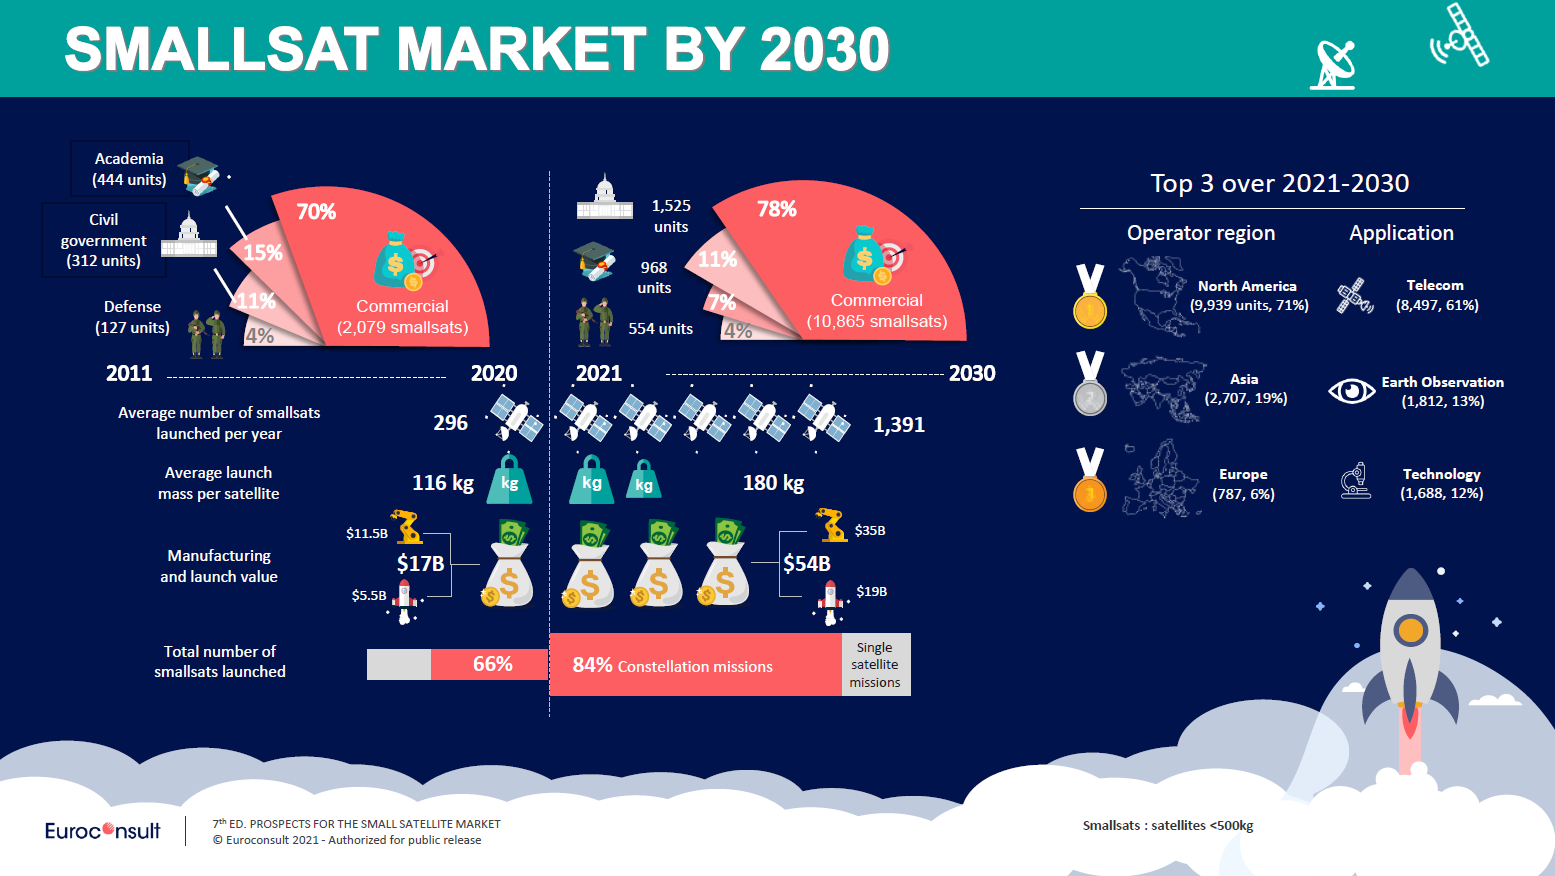
\includegraphics[width=1\textwidth]{Figures/EuroconsultSmallSatMarketBy2030.PNG}
    \caption{Small Satellite Market Survey 2021 \cite{euroConsult21}}
    \label{fig:smallSatMarket}
\end{figure}

%---------------------------------------------------------------------------
\begin{table}[!ht]
    \centering
    \caption{Current and planned Mega-Constelllations}
    \label{table:constellation}
    \resizebox{\textwidth}{!} {%
    \begin{tabular}{||c c c c||} 
    \hline
    Constellation & Organization & No. of Sats (full service est.) & altitude \\ [0.5ex] 
    \hline\hline
    Starlink\footnotemark{} & SpaceX &  42,000 & 580 km \\ 
    \hline
    OneWeb\footnotemark{} & OneWeb & 6372 & 1,200 km \\
    \hline
    Lightband\footnotemark{} & Telesat & 298 & 1,325 km \\
    \hline
    Kuiper\footnotemark{} & Amazon Kuiper LLC & 3,236 & 590 km, 610 km, 630 km \\
    \hline
    GuoWang\footnotemark{} & CASC & 12,992 & 508 km, 590 km, 600 km, 1,145 km \\ [1ex]
    \hline
    \end{tabular}
    }
\end{table}

\footnotetext[1]{Satellite mass definitions used in this dissertation are defined as follows: Cubesats $<$ 50 kg, Microsats 51 - 150 kg, Smallsats 151 - 500 kg} 
\addtocounter{footnote}{-4}
\footnotetext{\href{https://en.wikipedia.org/wiki/Starlink}{Wikipedia, "Starlink", May 5, 2021 [Online]}}
\addtocounter{footnote}{1}
\footnotetext{\href{https://en.wikipedia.org/wiki/OneWeb}{Wikipedia, "OneWeb", May 5, 2021 [Online]}}
\addtocounter{footnote}{1}
\footnotetext{\href{https://www.telesat.com/wp-content/uploads/2020/08/Telesat-Lightspeed-Defence.pdf}{Telesat, "Telesat LighSpeed", May 5, 2021 [Online]}}
\addtocounter{footnote}{1}
\footnotetext{\href{https://en.wikipedia.org/wiki/Kuiper_Systems}{Wikipedia, "Kuiper System", May 5, 2021 [Online]}}
\addtocounter{footnote}{1}
\footnotetext{\href{https://spacenews.com/china-is-developing-plans-for-a-13000-satellite-communications\-megaconstellation/}{Jones, A., "China is developing plans for a 13,000-satellite megaconstellation", SpaceNews, Apr. 21, 2021 [Online]}}
\addtocounter{footnote}{1}
\footnotetext{\href{https://spacenews.com/china-is-developing-plans-for-a-13000-satellite-communications\-megaconstellation/}{Liberatore, S., "SpaceX, OneWeb Satellites Come Within 190 Feet Of Each Other In Orbit", Space News, Apr. 9, 2021 [Online]}}

As of April 2021, Starlink has 1,383 satellites in orbit at 550 km altitude and OneWeb has 146 satellites in orbit 1,200 km altitude. On April 4th 2021, the StarLink and OneWeb satellites came within 190 feet of each other, triggering several red alerts from the US Space Force 18th Space Control Squadron to issue a warning to OneWeb who immediately maneuvered their 36 satellites launched recently on March 30th, 2021\footnotemark{}. This event exemplifies, 1) the very real danger of space asset collision leading to the Kessler Syndrome (ablation cascading) \cite{KesslerSyndrome78} without even accounting for the existing space debris that active space assets will have to avoid, and 2) the dependency of ground tracking measurements, data triage and human-in-the-loop decision making process space situational awareness. Clearly, the co-existence of these mega-constellations with existing and planned future space assets is extremely fragile.

%---------------------------------------------------------------------------
% DND, DRDC, Dark Arts
This concern has been been elevated in relevance within Canada's Department of National Defense (DND) to issue two Request for Information (RFI) in 2019 for the Surveillance of Space Ground (GBO) and Space based observation (SBO) \cite{dndRfi19a} - \cite{dndRfi19b}, a follow-on to the successful Sapphire microsatellite mission under the DND's Space Domain Awareness (SDA) Secure, Strong, Engaged Program. Sapphire is the first dedicated space-based RSO surveillance asset and has become an integral to the Canadian Space Operations Center's (CANSpOC) contribution to the Combined Space Ops (CSpOC) with US SPACECOM,  UK Space Operation Center (UK SpOC) and the Australian Space Operations Center (AUS SpOC). Concurrently, Defence Research and Development Canada (DRDC) issued an Innovation Call for Proposal  \cite{drdcCall19} for a space-based autonomous close-loop tracking Resident Space Object (RSO) surveillance microsatellite, a follow-on to NEOSat, under Space Technology Challenge No.15. One of five key technologies to be demonstrated is detection of RSOs within close orbital proximity of the microsatellite, reflecting the emphasis of an onboard space situational awareness (SSA). Such a capability would be essential in detecting hostile satellites in a space-to-space space-weapon framework as discussed in the "Protecting Space Systems from Counterspace Weapons" report by the Center for Strategic \& International studies \cite{darkArts21}. In addition, the listed active space-based defense strategy such as physically capturing the threatening object to disable or move it, which can also double as an inspector an on-orbit servicing satellite, requires a very robust onboard SSA coupled to a close proximity control system. A similar onboard SSA system would greatly benefit commercial mega-constellation space assets, providing greater ability to be self-aware of it's surrounding and to react autonomously in real-time.

% 4 GSO In-Orbit Servicing MEV-1.
In the case of an on-orbit servicing (OOS) system, previous concept studies and designs in last two decades \cite{tatschOss06,floresabadReviewSpaceRobotics20141} has finaly been realized by Northrop Grumman's Mission Extension Vehicle (MEV-1) \cite{mev121}. MEV-1 successfully rendezvoused with, refueled and and re-positioned the IntelSat 901 to GEO service in February 25th, 2020.  Northrop Grumman did it again with MEV-2, repeating the feat with Intelsat 10-02 on April 13th 2021\footnotemark[8]{}.
\footnotetext{\href{https://spacenews.com/mev-2-servicer-successfully-docks-to-live-intelsat-satellite/}{Rainbow, J., "MEV-2 servicer successfully docks to live Intelsat satellite", Space News, Apr. 12, 2021 [Online]}}
However, as highlighted by Harrison et al.\cite{darkArts21}, the host satellites are cooperative, similar to Space-X's Dragon capsule, Soyuz or ATV cargo spacecraft approaching and docking with the International Space Station (ISS) using proximity cameras in the visible-infrared spectrum and Light Detection and Ranging sensors (LiDARs) assisted by known physical markers \cite{OpromollaPose17}. These cooperative proximity sensing greatly improves the accuracy of rendezvous and docking operations. The distinguishing feature of a military defensive capability however, is the ability to conduct remote proximity and docking operations with an uncooperative or uncontrolled space object.These operations are extremely challenging when there is no consent from the host satellite or the satellite is lost, i.e. the target space object could make unexpected movements, may be tumbling, or may react unexpectedly to the docking if its automatic position and attitude control system remains engaged. 

 % 5 Debris Removal, Astroscale
The field of Active Debris Removal (ADR) missions architectures and technology development only came into prominence in 2007 when A Russian Briz-M booster stage exploded in orbit over South Australia generating 1,000 fragments \cite{bonnalAdr13}. Due to the nature of the uncooperative debris, vision technologies mentioned previously for 'dark' satellites will be limited in accuracy due to the various derbis size and characteristics \cite{limAdrVision13}.  The challenge of approaching a non-cooperative target has not deterred Astroscale's commercial vision to removed space debris. The Elsa-D microsatellite debris removal demonstrator, affectionately known as a "space sweeper", recently launched on March 22nd, 2021 \footnotemark{}, will move towards a test debris using GPS information, estimate its exact position and analyze its motion with (undisclosed) sensors and then will determine a path to approach the space junk before latching onto it using a magnetic docking plate. The space junk will be released before capturing another derbis and repeating the capture maneuver\cite{elsaD19}.
\footnotetext{\href{https://asia.nikkei.com/Business/Aerospace-Defense/Japan-s-Astroscale-launches-space-debris-removal-satellite}{Obe, M, "Japan's Astroscale launches space debris-removal satellite", Nikkei Asia, Mar. 22, 2021 [Online]}}

% 6 Lunar Gateway
Moving beyond GSO, NASA’s ambitious Artemis Program to land the first woman and the next man on the Lunar south pole by 2024 \cite{nasaArtermis20} and the goal to establish a Lunar gateway \cite{winternitzGpsLunarGateway19} by 2026 will see an increase of space traffic in Cis-Lunar space. A spacecraft bound for the Lunar Gateway will be guided by absolute trajectory knowledge with a certain level of accuracy, typically in the 100ths of km range. The GPS navigation experiment onboard the four Magnetospheric Multi-Scale (MMS) spacecraft had demonstrated the ability to receive GPS signals at extremely high altitudes, 4.6 times higher than GSO \cite{winternitzGpsLunarGateway19} and feasibility studies by Capuano et al.,  \cite{capuanoGpsLunarNav16} and Delépaut et. al, \cite{DelepautGpsLunarNav16} has proven that receiving GPS L1 signal is feasible within the moon transfer orbit. As the spacecraft approaches the Gateway to within meters in range to docking, precise relative position and orientation knowledge of the spacecraft is crucial in ensuring the spacecraft matches the the orientation of the Gateway. Although cooperative in nature; the approximately 400,000 km distance to be travelled  and line-of-sight of the deep-space communication link will result in delayed and limited command and telemetry operations. Hence the need for robust autonomous situational awareness and proximity system is imperative. This operational challenge is reinforced by the joint Canadian Space Agency/ MDA information session for the Lunar Gateway’s Canadarm3 \footnotemark{} that identified technical gaps for the robotic arm, i.e., situational awareness, proximity sensing, collision avoidance, supervise autonomy, and the need for AI autonomy.
\footnotetext{\href{https://mda.space/en/mda-launchpad/}{Canadian Space Agency-MDA, "Canadian Space Agency Canadarm3 information session", Jan 14, 2021}}

% 7 Asteroids
The field of asteroid exploration combines the two challenges of an uncooperative target and delayed communication link to Earth as evident in both the HAYABUSA (MUSE-C) mission \cite{Kobayasi3DofPoseAsteroid15} and OSIRIS-REX \cite{leonarOsirusRex19}. Both spacecraft missions successfully returned asteroid samples relied heavily on visual and lidar images for relative position and orientation of the asteroid to the spacecraft with careful, and complex, navigation and proximity events to "landing and descent" of the Asteroid sample tool. In the case of OSIRIS-REX, an onboard optical navigation system that compares observed images to a set of asteroid terrain models which are rendered in real-time from a catalog stored in memory on the flight computer, and onboard knowledge of the spacecraft state is then updated by a Kalman filter using the measured residuals between the rendered reference images and the actual observed images \cite{lorenzOsirusRexAutoNav}.      

% 7 Formation Flying
Situational awareness and proximity sensing are also critical in satellite formation flying (FF). Measurement missions that require precise baseline separations such as synthetic aperture radar, gravimetry, and deep-space observation, are significantly enhanced when the measurement baseline is distributed to individual space assets \cite{frasierAdaptiveKF18}. These assets will need to know their relative position and orientation with respect to each other, sometimes down to the cm range to ensure tight formation flying. Similar to operations in Cis-lunar space, future deep-space science missions like LISA located at 0.35 AU from Earth \cite{amatoFormationFlying19} will encounter similar communication delays with even more stringent attitude requirements. Hence an autonomous and adaptive relative navigation and attitude estimator ensures intelligent and timely responses for safe operations in the absence of human decision making processes.   

The underlining denominator for all scenarios outlined for a spacecraft with respect to another, is a close-loop event that can be synthesized into three processes; 1) situational or proximity awareness (sense), 2) task planning (reasoning or control); and 3) task execution (actuation). Within situational or proximity awareness, the term pose estimation is frequently used. Specifically, pose represents the combination of the \textit{position} and \textit{orientation} of an object \textit{relative} to another object, or reference point within a defined coordinate system \cite{PrezVillar2017SpacecraftPE}.  Pose estimation is the specific task of determining the pose of an object using proximity sensors. The pose estimation are distinct for each scenario that the spacecraft needs to operate, which can be summarized as follows:
\begin{enumerate}
    \item Cooperative and non-cooperative collision avoidance; 
    \item Cooperative and non-cooperative rendezvous; 
    \item Cooperative contact and non-cooperative contact; and
    \item Formation Flying.
\end{enumerate}

The pose estimator designed for one environment is not necessarily applicable to another. Hence, the motivation of this research is to explore and develop a dynamic, adaptive and autonomous space asset pose estimator that is agnostic to any space scenario.

%%%%%%%%%%%%%%%%%%%%%%%%%%%%%%%%%%%%%%%%%%%%%%%%%%%%%%%%%%%%%%%%%%%%%%%%%%%%
%  Problem Statement
%%%%%%%%%%%%%%%%%%%%%%%%%%%%%%%%%%%%%%%%%%%%%%%%%%%%%%%%%%%%%%%%%%%%%%%%%%%%
\section{Problem Statement}\label{CHAP1_2}

Pose sensors mounted on a space asset provide physical measurements that are mapped to the position and orientation of the space asset's body frame relative to another frame, whether it is a Earth centered fixed inertial (ECI) or another spacecraft body reference frame \cite{PrezVillar2017SpacecraftPE}. The scenario discussed in the previous section is more suitably labeled as relative pose estimation using different definitions of dynamic and kinematic equations that define the relation between the two spacecraft body frames \cite{OpromollaPose17}.  In generally; the process to determine the kinematic and dynamic position and orientation relationship can be establish using there main approaches \cite{landisMarkleyFundamentalsOfADCSSpacecraft15}:
\begin{enumerate}
    \item deterministic (determination);
    \item probabilistic (estimation); and   
    \item combination of deterministic and probabilistic approaches. 
\end{enumerate}

Note the term determination is broadly used in literature to include estimation. There is, however, a clear distinction where determination is solely a deterministic algebraic vector process, whereas estimation is an indirect vector modelling process \cite{Dhahbane2021AttitudeDA}. This dissertation will use the broad definition of determination except when a clear distinction is required. 

Both the deterministic and probabilistic approaches are reliant on sensor performances that depend on the physical principal of the system and quality of the components. For example, visual cameras are dictated by the physical optics (aperture size, focal length, lenses curvature and surface finish), detectors (pitch length, radiometric sensitivity) and read-out electronics (integration time, analogue digital conversion, clock frequency). For a Global Navigation Satellite System (GNSS) receiver mounted on both space assets to determine relative position, i.e. differential GNSS techniques, the position telemetry depend on the performance of the GNSS antenna gain, temperature and line noise, and electronic  acquisition, tracking and FPGA navigation processing. These sensors are cost sensitive, where better performance detectors and electronics will cost higher \cite{hashim2021attitude}. The inherent sensor noise that exist decreases pose determination accuracy. Hence a deterministic pose approach is shackled to the sensor noise unless algorithm data processing and filtering are employed to improve accuracy\cite{OpromollaPose17}.

A probabilistic approach uses probability techniques to minimize the difference between the state models (the estimate) to the actual sensor measurements, i.e. a cost function regression exercise. The ubiquitous Kalman filter (KF) used in  aerospace guidance, navigation, attitude and orbit estimation is simply a weighted recursive least square coupled to a state space dynamic model 'propelled' by propagating and correcting the process and measurement noise variance \cite{franklinDigitalControl97}. The recursive framework is important for real-time implementation onboard the spacecraft, versus batch post processing and the statistical approach assumes a normal Gaussian distribution for both the process and measurement noise - which are idealistic in reality. For pose estimation, the state dynamics are non-linear. Similarly the pose sensor physical measurements mapped to the estimated states can be non-linear, which violates the linear assumption of the Kalman Filter. Hence a local linearization of the state transition matrix and the measurement matrix are required at each time-step. This approach is sup-optimal as the state transition matrix for example relies on a Taylor series expansion and the idealistic Gaussian noises. In most implementation cases; the Taylor series is truncated and only the first two dominant terms are considered but the Gaussian noises are still assumed \cite{franklinDigitalControl97,cavenagoEkfHighOrder19}. This version is called the Extended Kalman filter (EKF) and serves well in most benign orbit position and orientation (attitude) estimation. The dynamic range of the space asset operating in the three broad scenarios described in Section \ref{CHAP1_1} from km to m in range however, produces a time variant noise that in most formulations of the EKF are considered static in nature. This limits the utilization of the EKF pose estimation to within well defined noise envelopes i.e., a near range environment. Unlike co-operative targets that would provide active markers \cite{OpromollaPose17}, space assets approaching non-cooperative targets are solely dependant on the pose sensor performance. Ideally, pose estimation should be inclusive of both the near range and far range pose sensor measurement environment i.e., as the spacecraft approaches from a few kilometers to within meters or centimeters for direct contact. This essentially improves situational awareness during all phases of the space asset approaching the target, improving task planning and optimizing task execution i.e., reducing delta-V, the propellant required to complete the entire closed-loop process for estimating the proximity of other space assets, rendezvous and docking, and formation flying.


%%%%%%%%%%%%%%%%%%%%%%%%%%%%%%%%%%%%%%%%%%%%%%%%%%%%%%%%%%%%%%%%%%%%%%%%%%%%
%  Previous Work
%%%%%%%%%%%%%%%%%%%%%%%%%%%%%%%%%%%%%%%%%%%%%%%%%%%%%%%%%%%%%%%%%%%%%%%%%%%%
\section{Previous Work}\label{CHAP1_3}
The earliest pose estimation studies, or in more generic terms, relative navigation, stems from the early Gemini missions \cite{chamberlinGemini64} which led to the Apollo missions \cite{youngApollo70} for orbital rendezvous, docking and control (RODC). This is essentially cooperative rendezvous and contact between two spacecrafts as discussed in Section \ref{CHAP1_1}. These early RODC missions rely on Radio-Frequency (RF) antennas installed on-board both the chaser and the target. The RF frequencies were exploited to obtain range, range-rate, Line-of-sight (LOS) angles and relative attitude parameters within several kilometers of precision \cite{fehse_2003, woffidenRez07}. RODC in general consists of  several phases that can be generalized in  Figure \ref{fig:rendezvousPhase}. During the phasing period, absolute navigation is in operations and as the chaser enters the close-range rendezvous phase, relative navigation is initiated. The homing and closing sub-phases ranges in kilometers and as the spacecraft enters the final approach phase to the target, relative position, velocity, attitude and angular rate information are required by the chaser to ensure a  straight light approach to docking. These legacy RF systems used in RODC, however, are massive and have now been superseded with on-board Global Positioning System (GPS) receivers used spacecraft missions such as GRACE \cite{yangInterSatelliteGrace13} and PRISMA \cite{dAmicoPrisma11} with near real-time relative distance precision within 4.2 cm 3D RMS and 5.0 cm 3D RMS respectively. These missions are not RODC however and in fact are true FF operational missions. PRISMA in particular reported \cite{bodinPrisma12} a relative bearing (attitude) between the MANGO-TANGO spacecraft to be less than 0.1\textdegree.
%---------------------------------------------------------------------------
\begin{figure}[ht]
    \centering
    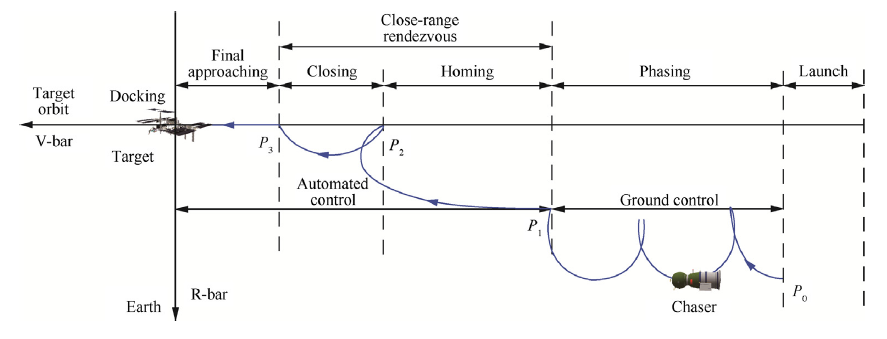
\includegraphics[width=1\textwidth]{Figures/LuoSurveyOfRelativeNavigation.PNG}
    \caption{Generic spacecraft rendezvous and docking phases \cite{luoSurvey13}}
    \label{fig:rendezvousPhase}
\end{figure}
%---------------------------------------------------------------------------

As described by Luo et al. \cite{luoSurvey13}, the navigation sensors can be divided into two categories: relative and absolute. Absolute navigation sensors determines the spacecraft position and attitude in the inertial frame using navigation equipment, inertial measurement units and optical attitude sensors. Relative sensors on the other hand determines the chaser's position, velocity, attitude and angular rate with respect to the target using relative navigation equipment, microwave radars, lidars, optical imaging sensors and television cameras. Oppromila et al.\cite{OpromollaPose17}, categorizes these sensors as electro-optical sensors in a well-defined taxonomy's as shown in Figure \ref{fig:taxonomyEo}. 
%---------------------------------------------------------------------------
\begin{figure}[ht]
    \centering
    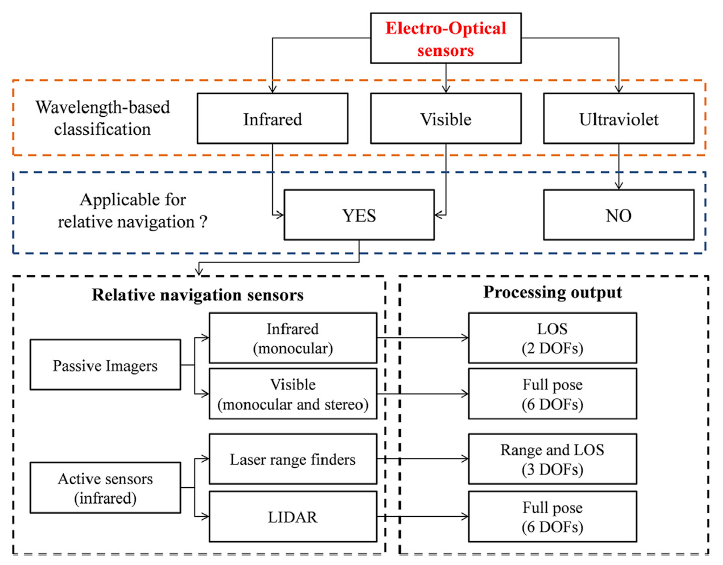
\includegraphics[width=1\textwidth]{Figures/OppromolaTaxanomyPoseSensors.PNG}
    \caption{Taxanomy of Electo-Optical relative pose sensors \cite{OpromollaPose17}}
    \label{fig:taxonomyEo}
\end{figure}
%---------------------------------------------------------------------------
The determination of the relative pose states are either deterministic instantaneous from sensor outputs or the filtered historic outputs of these measurements, i.e., estimation as mentioned in Section \ref{CHAP1_2}. For the former, relative distance, velocity and attitude can be extracted directly based on geometric extraction of feature points monocular visual system images \cite{aghiliPoseVision10, leiPoseSlam19, sharmePoseNonC17a, ShijieMono10}. Sharma et. al, in particular  dealt with non-cooperative target images \cite{sharmePoseNonC17a}. For the latter, the Extended Kalman filter (EKF) is the most widely used filter algorithm for relative navigation \cite{dAmicoPrisma11,karlgaardAdaptiveEkf11} and utilizes either Clohessy–Whiltshire (C–W) equations \cite{CW} for circular orbits or Tschauner and Hempel (T-H) equations \cite{Tschauner65} for elliptical orbits. The popularity of the EKF for pose estimation requires further treatment in this dissertation. 

%Kim et. al, \cite{kimPoseGyroYY} formulated the EKF using line-of-sight measurement with gyro measurements and an EKF.   

%during these phases are mostly done either by (1) angles-only relative measurement or (2) by image information. For the former; maximum measuring distances are limited to a few tens of kilometers for non-cooperative target rendezvous as distance measurements have large uncertainties. 
%For the latter, image measurements come in the form of charge-coupled device binocular or monocular vision measurements. Using monocular vision measurement will require the use of the Clohessy–Whiltshire (C–W) or Hill equations, for circular equations and Tschauner and Hempel (T-H) equations for elliptical orbits. 

%As expected the EKF has been the major filter algorithm used for rendezvous navigation. Particle filters was also employed in a few studies, although onboard implementation feasibility can be challenging given the computational recursion of the algorithm itself \cite{}. An adaptive method to automatically tune the Kalman filter by estimating measurement and processing noise co variance to improve the robustness of the filter for an elliptical rendezvous navigation problem had been investigated. 

\subsection{Extended Kalman filter}\label{CHAP1_3_1}
The EKF has been the workhorse for many aerospace guidance, navigation and attitude determination systems since its inception in the 1960's. The EKF is the linearized version of the linear Kalman Filter formulated by Rudolph Kalman in his seminal paper "A New Approach to Linear Filtering and Prediction Problems" \cite{Klmn1960ANA}. The EKF was specifically formulated to resolve the measurement gaps encountered during the Apollo Service Module (and the attached Descent Module when outbound) during the 76 hrs Moon Transfer Orbit (MTO) trajectory. In particular; the EKF was used to determine when the Mid-Correction burns were required during transit. For history buffs, Grewal \cite{grewalKFHistory10} provides a very refreshing read on the beginnings of the EKF, its roots in spacecraft guidance and navigation, and the proliferation to GNSS and particular Inertial Navigation systems for terrestrial applications. In essence, the EKF is essentially (1) predicting  future states based on available inputs and assumptions \cite{hashim2021attitude} and (2) reducing the workload of human decision making, in essence a rudimentary sense of autonomy. The robustness of the EKF has been applied for spacecraft pose estimation, with numerous research and onboard implementations on satellites since the early 2000s, such as GRACE \cite{yangInterSatelliteGrace13}, PRISMA \cite{dAmicoPrisma11} and the Can-X4 and Can-X5 satellites \cite{boninCanX}.

These techniques however assumes all state and measurement noises are Gaussian and white, which are the foundation of the EKF, when in reality they may not be. Hence the EKF, will still behave poorly if the system is non-Gaussian. For example, the execution of an impulsive thrust results in state transitional acceleration that if not accounted for in the EKF dynamics, will lead to divergence of the estimated states in the corrector phase. 

The adaptive EKF filter has also been studied by Frasier for relative formation flying with an excellent treatment of the formulation and simulation \cite{frasierAdaptiveKF18}. Similarly, Woffinden et al., developed an adaptive Hurber-based EKF to provide better covariance adaption to avoid filter divergance and the varying relative dyanmic elliptical FF \cite{woffidenRez07}.


In the last decade, researchers have pivoted to Artificial Intelligence (AI) for a non-Gaussian navigation estimator \cite{}. 


\subsection{Artificial intelligence}\label{CHAP1_3_2}
The evolution of Artificial Intelligence (AI), or more explicitly Machine Learning, has accelerated the transition of repetitive analytical task to be completed autonomously and within shorter time-frames. At the core of Machine Learning (ML) is the minimization of the cost function between a states or states that defines the model and the associated measurement or measurements, i.e. a linear regression or logistic regression process. Given that no dynamical models are required, unlike the KF / EKF, ML approaches, ML can prove an alternate approach to improve the pose estimation as defined previously. Neural-networks (NN) is a type of ML that mimics the human brain and expands on cost minimization process by modelling a network of state nodes, weighted and triage using an activation function (sometimes called a perceptron) at each layer to find the best possible outcome \cite{yangML21}.
%%
The work on Artificial Intelligence (AI), Machine Learning (ML) and its Neural Network (NN) subset as well as Deep Learning (DL) are continuously evolving at a daily rate. It would be a herculean task to present the evolution of this field of study. 


The nascent spacecraft pose estimation using ML/NN have found to be limited to mostly vision based measurements. Sharma \cite{sharmePoseNonCYYb} proceeded to develop a Convolutional Neural Network (CNN) applied to the monocular images for POSE estimation. Similarly, Prenca \cite{prencaDlPosePhotorealistic19} developed a probabilistic quaternion fitting pose estimator using Deep Learning. Mihai \cite{mihaiPoseAnn20} investigated the use of an onboard Artificial Neural Network (ANN) satellite orbit estimator with coefficients pre-trained using a 3-week training data set with mean errors less than a kilometer. The paper acknowledges that maintenance of these coefficient(s) is required, i.e. the need for periodic training to update the coefficients. To the best of the author's knowledge, the work by Forghani's is the only research comparing a satellite orbit estimation performance using an EKF only versus an on-line Neural Network only approach. His researched concluded that the NN provided a better orbit estimate compared to the EKF for the CHAMP satellite orbit parameters using an Earth tracking ranging station, including a simulated measurement outage. Both methods could cope well with ranging data outages, with the NN showing less estimation error than the EKF. However, none of these aforementioned studies involve the fusion of an EKF with a NN for POSE estimation.

Nevertheless, terrestrial ground robotic research have explored the combination of EKF and NN for trajectory estimation. Bai's \cite{baiKf20} paper in particular has shown a improved trajectory estimation of a robotic rover traversing an elliptical race track using a tightly coupled trained onboard KF-ANN architecture. Unlike other terrestrial implementation research that performs EKF estimation that feeds into a ANN to improve performance or vice-versa, Bai's approach uses a two intermediate node ANN integrated into the KF predictor-corrector recursive loop. Node 1 minimizes the errors of the predicted KF where the results are then fed back into the KF measurement update. Node 2 then minimizes the errors after the KF measurement updated before sending the estimates back into the KF state prediction. The ANN uses a nonlinear aurotoregressive model with exogenous input (NARX) which basically takes the historic outputs and the associated historic inputs into the ANN. This approach is similar to the one used by Forghani \cite{}.     

%%
ML however are not without its drawbacks. The probabilistic nature does not always guarantee the confidence of the approach in an industry that is risk-adverse, particularly when human lives are at stake.  Perhaps the solution to improve the limitations of a dynamic pose estimator lies in the marriage of an EKF and NN approach that would allow a common new pose estimator to operate in any environment and with any pose sensor. This research sets out to solve this problem. 
 
%%%%%%%%%%%%%%%%%%%%%%%%%%%%%%%%%%%%%%%%%%%%%%%%%%%%%%%%%%%%%%%%%%%%%%%%%%%%
%  Objectives
%%%%%%%%%%%%%%%%%%%%%%%%%%%%%%%%%%%%%%%%%%%%%%%%%%%%%%%%%%%%%%%%%%%%%%%%%%%%
\section{Thesis Objectives}\label{CHAP1_4}

The goal of this research is to develop a modular autonomous enhanced situational awareness technology for a space asset pose.

The primary objective of this thesis is to develop a near real-time EKF-NN for estimating the relative pose of a chaser spacecraft with respect to a tumbling uncooperative target spacecraft. Specifically, the EKF process and measurement noise covariances will be adapted using a Neural Network (NN), as function of the varying separation between both vehicles throughout a representative mission profile; from far-range approach to close-range rendezvous and contact (see Figure \ref{fig:rendezvousPhase}). The EKF-NN design, referred to as the Space Machine Attitude and oRbit inTelligence (SMART), assumes arbitrary computer vision algorithms will provide a rough pose measurement inputs (computer vision algorithms will not be the focus of this research). The expectation is that SMART will operate in any pose scenario, not be bounded by a pre-defined dynamic model and will only be constrained by the onboard processor performance, timing, sampling frequencies, and sensor characteristics.

%Secondary objective: Research and develop an autonomous close-loop target tracking provided by the SMART, using %Reinforced Learning (RL). 

%%%%%%%%%%%%%%%%%%%%%%%%%%%%%%%%%%%%%%%%%%%%%%%%%%%%%%%%%%%%%%%%%%%%%%%%%%%%
% Methodology
%%%%%%%%%%%%%%%%%%%%%%%%%%%%%%%%%%%%%%%%%%%%%%%%%%%%%%%%%%%%%%%%%%%%%%%%%%%%
\section{Methodology}\label{CHAP1_5}

%\begin{enumerate}
%    \item algorithm design in MATLAB (EKF only, EKF and NN, etc.)
%    \item simulation analysis with 3 scenarios (eg., docking with cooperative target, capture of %uncooperative target, approach with vision-only information),and
%    \item hardware-in-the-loop demonstration (describe the facility)
%\end{enumerate}

This research will follow subset of a space industrial ‘V’ requirements definition, analysis, development and verification in a software-based simulated environment followed by a hardware-in-the-loop (HIL) test bench. 

This research is initiated with a literature review to define the motivation, problem statement, previous work and objectives. A set of preliminary technical performance metrics (TPM) will be defined for the three operational environments. A step-by-step  algorithm will be developed in MATLAB, (one state KF, linear regression, NN stand-alone and combined KF-NN) followed by the completed 6  state / 6 degrees of freedom (DOF) pose algorithm (EKF, EKF-NN). In parallel a simplified relative orbit and attitude propagator in MATLAB will be developed to preliminary test the EKF-NN. A complete Satellite Toolkit rendezvous and docking scenarios, e.g. docking with a cooperative target, capture of uncooperative target) will be established to generate relative pose information to be used as the truth and to emulate a pose sensor inputs (baseline  vision-only information) to verify the EKF-NN in a higher fidelity simulated environment. 

The next phase would be to deploy the algorithm in Carleton University’s air-bearing chaser-target system that contains a NVIDIA AI capable processor with a basic camera and potentially integrating York’s sun sensor and star tracker (in development) to test pose estimation and uncooperative target tracking in 3 DOF (2 DOF translation, 1 DOF rotation).The performance of this HIL will verify a real-time implementation of the EKF-NN algorithm in a real-world like terrestrial environment.

%%%%%%%%%%%%%%%%%%%%%%%%%%%%%%%%%%%%%%%%%%%%%%%%%%%%%%%%%%%%%%%%%%%%%%%%%%%%
% Schedule
%%%%%%%%%%%%%%%%%%%%%%%%%%%%%%%%%%%%%%%%%%%%%%%%%%%%%%%%%%%%%%%%%%%%%%%%%%%%
\section{Schedule}\label{CHAP1_6}
The preliminary research schedule will be aligned to seven (7) academic terms with three journal papers scheduled in term 3, 5 and 6 (TBD). The dissertation will be generated in term 1 and completed by term 7.
\begin{enumerate}
    \item Term 1 (Spring 21):  Perform literature review and generate chapter 1 of dissertation. Develop test algorithms.
    Deliverable: D1.1 Dissertation Chapter 1, D2.1: Test built

    \item Term 2 (Summer 21):  Develop preliminary EKF-NN. Development pose (6 DOF) simulator.  
    Deliverable: D1.2 Dissertation Chapter 2, D2.2 AttDet Algorithm built 

    \item Term 3 (Fall 21): Optimize EKF-NN. Development pose EO scenario.  
    Deliverable: D1.3 Dissertation Chapter 3, D2.3 AttDet Algorithm built, D3.3 Journal paper 1 draft
    
    \item Term 4 (Winter 22): Deploy the algorithm in HIL Testbench
    Deliverable: D1.4 Dissertation Chapter 3, D2.4 AttDet Algorithm built, D3.3 Journal paper 1 draft
    

    \item Term 5 (Spring 22): Review of data against TPM and optimize algorithm. Retest if needed. 
    Deliverable: D1.4 Dissertation Chapter 4, D2.5 AttDet Algorithm built, D3.5 Journal paper 1 final

    \item Term 6 (Summer 22): Complete Dissertation, update algorithm, generate journal paper 
    Deliverable: D1.5 Dissertation Chapter 5, D2.6 AttDet Algorithm built, D3.6 Journal paper 2 draft

    \item Term 7 (Fall 22): Complete Dissertation, update algorithm, generate journal paper
    Deliverable: D1.6 Dissertation Chapter 6, D2.7 AttDet Algorithm built, D3.7 Journal paper 2 final

    \item Term 8 (Winter 23): Complete Dissertation, update algorithm, generate journal paper
    Deliverable: D1.7 Dissertation Chapter 7, D3.8 Journal paper 3 draft and final

\end{enumerate}

%%%%%%%%%%%%%%%%%%%%%%%%%%%%%%%%%%%%%%%%%%%%%%%%%%%%%%%%%%%%%%%%%%%%%%%%%%%%
% Progress to Date
%%%%%%%%%%%%%%%%%%%%%%%%%%%%%%%%%%%%%%%%%%%%%%%%%%%%%%%%%%%%%%%%%%%%%%%%%%%%

\section{Progress to Date}\label{CHAP1_7}
\begin{enumerate}
    \item Term 1 (Spring 21):  Perform literature review and generate chapter 1 of dissertation. Develop test algorithms. DONE
    Deliverable: D1.1 Dissertation Chapter 1, D2.1: Test built

\end{enumerate}

%%%%%%%%%%%%%%%%%%%%%%%%%%%%%%%%%%%%%%%%%%%%%%%%%%%%%%%%%%%%%%%%%%%%%%%%%%%%
% Summary and Future Work
%%%%%%%%%%%%%%%%%%%%%%%%%%%%%%%%%%%%%%%%%%%%%%%%%%%%%%%%%%%%%%%%%%%%%%%%%%%%
\section{Summary and Future Work}\label{CHAP1_8}
Chapter 1 of the dissertation, i.e. literature review to define the motivation, problem statement, previous work and objectives have been defined. The schedule and deliverables have been drafted in this progress report. The next step is to develop the preliminary EKF-ANN and the reference attitude and body rate (6 DOF) simulator. Depending on the progress of the research, availability of this part-time student and Covid pandemic restricting HIL access, the three journal papers will be pull forward if favourable opportunities arise for the to-be-identified journals. 

%%%%%%%%%%%%%%%%%%%%%%%%%%%%%%%%%%%%%%%%%%%%%%%%%%%%%%%%%%%%%%%%%%%%%%%%%%%%
%  Thesis Organization
%%%%%%%%%%%%%%%%%%%%%%%%%%%%%%%%%%%%%%%%%%%%%%%%%%%%%%%%%%%%%%%%%%%%%%%%%%%%

%\section{Organization}\label{CHAP1_5}

%\lipsum